The data in Table 6.8 were collected to test two psychological models of numerical cognition.
Does the processing of numbers depend on the way the numbers are presented (words, Arabic digits)?
Thirty-two subjects were required to make a series of quick numerical judgments about two numbers presented as either two number
words (``two,'' ``four'') or two single Arabic digits (``2,'' ``4'').
The subjects were asked to respond ``same'' if the two numbers had the same numerical parity (both even or both odd) and ``different'' if the two numbers had a different parity (one even, one odd).
Half of the subjects were assigned a block of Arabic digit trials, followed by a block of number word trials, and half of the subjects received the blocks of trials in the reverse order.
Within each block, the order of ``same'' and ``different'' parity
trials was randomized for each subject.
For each of the four combinations of parity and format, the median reaction times for correct responses were recorded for each
subject.
Here
\begin{align*}
    X_{1} &= \text{median reaction time for word format-different parity combination} \\
    X_{2} &= \text{median reaction time for word format-same parity combination} \\
    X_{3} &= \text{median reaction time for Arabic format-different parity combination} \\
    X_{4} &= \text{median reaction time for Arabic format-same parity combination}
\end{align*}

\begin{enumerate}[label= (\alph*)]
    \item Test for treatment effects using a \textit{repeated measures design}. Set $\alpha = .05$.
    
    Using what's in 6.2, that starts on page 273, and use the formula (6--16) from page 280.
    
    \[
        H_{0}: \textbf{C} \bm{\mu} = \textbf{0}
        \hspace{0.2cm}\text{versus}\hspace{0.2cm}
        H_{1}: \textbf{C} \bm{\mu} \ne \textbf{0}
    \]

    \[
        \textbf{C}
        =
        \begin{bNiceArray}{rrrr}
            -1 &  1 &  0 & 0 \\
             0 & -1 &  1 & 0 \\
             0 &  0 & -1 & 1
        \end{bNiceArray}
    \]

    \[
        \bar{\textbf{x}}
        =
        \begin{bNiceArray}{r}
            967.563 \\
            875.609 \\
            825.313 \\
            710.938
        \end{bNiceArray}
        \hspace{0.2cm}
        \textbf{S}
        =
        \begin{bNiceArray}{rrrr}
            36178.351 & 25936.727 & 18447.569 & 15909.238 \\
            25936.727 & 22597.754 & 14261.731 & 14115.934 \\
            18447.569 & 14261.731 & 18487.819 & 11799.730 \\
            15909.238 & 14115.934 & 11799.730 & 13001.399
        \end{bNiceArray}
    \]

    \begin{align*}
        T^{2}
        & =
        n
        {\left(\textbf{C}\bar{\textbf{x}}\right)}^{\prime}
        {\left(\textbf{C}\textbf{S}\textbf{C}^{\prime}\right)}^{-1}
        \left(\textbf{C}\bar{\textbf{x}}\right)
        \\
        & =
        \begin{multlined}[t]
        \begin{bNiceArray}{rrr}
            -91.953 & -50.297 & -114.375
        \end{bNiceArray}
        \\
        \times
        \begin{bNiceArray}{rrr}
             0.000166778541  &  -0.00002657034 & -0.000072607336 \\
            -0.000026570341 &   0.000144344912 &  0.000127750060 \\
            -0.000072607336 &   0.000127750060 &  0.000254696501
        \end{bNiceArray}
        \\
        \times
        \begin{bNiceArray}{r}
             -91.953 \\
             -50.297 \\
            -114.375  
        \end{bNiceArray}
        \end{multlined}
        \\
        & =
        153.7275
    \end{align*}

    \[
        \frac{(n-1)(q-1)}{(n-q+1)}
        F_{q-1, n-q+1}\left(\alpha\right)
        =
        \left(\frac{93}{29}\right)
        3.607
        =
        11.567
    \]

    \[
        T^{2}
        =
        153.7275
        >
        \frac{(n-1)(q-1)}{(n-q+1)}
        F_{q-1, n-q+1}\left(\alpha\right)
        =
        11.567
    \]
    \text{ so we'd reject the null hypothesis that }
    $\textbf{C}\bm{\mu}
    =
    \textbf{0}$.

    \item Construct 95\% (simultaneous) confidence intervals for the contrasts representing
    the number format effect, the parity type effect and the interaction effect. Interpret
    the resulting intervals.

    Using formula (6--18) on page 281:
    \[
        \textbf{c}^{\prime}\bm{\mu}\text{: }
        \textbf{c}\bar{\textbf{x}}
        \pm
        \sqrt{
            \frac{(n-1)(q-1)}{(n-q+1)}
            F_{q-1, n-q+1}\left(\alpha\right)
        }
        \sqrt{
            \frac{\textbf{c}^{\prime}\textbf{S}\textbf{c}}{n}
        }
    \]

    \textbf{Number format effect}

    \[
        \textbf{c}_{1}
        =
        \begin{bNiceArray}{r}
            -1 \\
            -1 \\
             1 \\
             1
        \end{bNiceArray}
    \]


    \[
        \textbf{c}_{1}^{\prime} 
        \bar{\textbf{x}}
        =
        \begin{bNiceArray}{rrrr}
            -1 & -1 & 1 & 1
        \end{bNiceArray}
        \begin{bNiceArray}{r}
            967.563 \\
            875.609 \\
            825.313 \\
            710.938
        \end{bNiceArray}
        =
        -306.9219
    \]
 
    The 95\% confidence interval for the number format effect contrast 
    $\textbf{c}_{1}^{\prime}\bm{\mu}$ is:
    \begin{align*}
         \textbf{c}_{1}^{\prime}\bm{\mu}\text{:}
         &
        \textbf{c}_{1}\bar{\textbf{x}}
        \pm
        \sqrt{
            \frac{(n-1)(q-1)}{(n-q+1)}
            F_{q-1, n-q+1}\left(\alpha\right)
        }
        \sqrt{
            \frac{\textbf{c}_{1}^{\prime}\textbf{S}\textbf{c}_{1}}{n}
        }
        \\
        & =
        \left(\bar{x}_{3} + \bar{x}_{4}\right)
        -
        \left(\bar{x}_{1} + \bar{x}_{2}\right)
        \pm
        \sqrt{
            \frac{(n-1)(q-1)}{(n-q+1)}
            F_{q-1, n-q+1}\left(\alpha\right)
        }
        \sqrt{
            \frac{\textbf{c}_{1}^{\prime}\textbf{S}\textbf{c}_{1}}{n}
        }
        \\
        & =
        -306.9219
        \pm
        \sqrt{
            \frac{(32-1)(4-1)}{(32-4+1)}
            F_{4-1, 32-4+1}(0.05)
        }
        \sqrt{
            \frac{40269.2921}{32}
        }
        \\
        & =
        -306.9219
        \pm
        \sqrt{11.5679}
        \sqrt{
            \frac{40269.2921}{32}
        }
        \\
        & =
        -306.9219
        \pm
        120.6532
        \\
        & =
        \left[-427.58, -186.27\right]
    \end{align*}
   
    With 95\% confidence, the mean arabic digits score is between 186 and 428 points lower than that of word scores.

    \textbf{Parity type effect}
  
    \[
        \textbf{c}_{2}
        =
        \begin{bNiceArray}{r}
             1 \\
            -1 \\
             1 \\
            -1
        \end{bNiceArray}
    \]

    \[
        \textbf{c}_{2}^{\prime} 
        \bar{\textbf{x}}
        =
        \begin{bNiceArray}{rrrr}
            1 & -1 & 1 & -1
        \end{bNiceArray}
        \begin{bNiceArray}{r}
            967.563 \\
            875.609 \\
            825.313 \\
            710.938
        \end{bNiceArray}
        =
        206.3281
    \]
 
    The 95\% confidence interval for the type effect contrast 
    $\textbf{c}_{2}^{\prime}\bm{\mu}$ is:
    \begin{align*}
         \textbf{c}_{2}^{\prime}\bm{\mu}\text{:}
         &
        \textbf{c}_{2}\bar{\textbf{x}}
        \pm
        \sqrt{
            \frac{(n-1)(q-1)}{(n-q+1)}
            F_{q-1, n-q+1}\left(\alpha\right)
        }
        \sqrt{
            \frac{\textbf{c}_{2}^{\prime}\textbf{S}\textbf{c}_{2}}{n}
        }
        \\
        & =
        \left(\bar{x}_{1} + \bar{x}_{3}\right)
        -
        \left(\bar{x}_{2} + \bar{x}_{4}\right)
        \pm
        \sqrt{
            \frac{(n-1)(q-1)}{(n-q+1)}
            F_{q-1, n-q+1}\left(\alpha\right)
        }
        \sqrt{
            \frac{\textbf{c}_{2}^{\prime}\textbf{S}\textbf{c}_{2}}{n}
        }
        \\
        & =
        206.3281
        \pm
        \sqrt{
            \frac{(32-1)(4-1)}{(32-4+1)}
            F_{4-1, 32-4+1}(0.05)
        }
        \sqrt{
            \frac{19577.4776}{32}
        }
        \\
        & =
        206.3281
        \pm
        \sqrt{11.5679}
        \sqrt{
            \frac{19577.4776}{32}
        }
        \\
        & =
        206.3281
        \pm
        84.1260
        \\
        & =
        \left[122.20, 290.45\right]
    \end{align*}
   
    With 95\% confidence, the mean ``different'' numeric parity score is between 122 and 290 points ``same'' than that of word scores.

    \textbf{interaction effect}

    \[
        \textbf{c}_{3}
        =
        \begin{bNiceArray}{r}
             1 \\
            -1 \\
            -1 \\
             1
        \end{bNiceArray}
    \]

    \[
        \textbf{c}_{3}^{\prime} 
        \bar{\textbf{x}}
        =
        \begin{bNiceArray}{rrrr}
            1 & -1 & -1 & 1
        \end{bNiceArray}
        \begin{bNiceArray}{r}
            967.563 \\
            875.609 \\
            825.313 \\
            710.938
        \end{bNiceArray}
        =
        -22.422
    \]
 
    The 95\% confidence interval for the interaction effect contrast 
    $\textbf{c}_{3}^{\prime}\bm{\mu}$ is:
    \begin{align*}
         \textbf{c}_{3}^{\prime}\bm{\mu}\text{:}
         &
        \textbf{c}_{3}\bar{\textbf{x}}
        \pm
        \sqrt{
            \frac{(n-1)(q-1)}{(n-q+1)}
            F_{q-1, n-q+1}\left(\alpha\right)
        }
        \sqrt{
            \frac{\textbf{c}_{3}^{\prime}\textbf{S}\textbf{c}_{3}}{n}
        }
        \\
        & =
        \left(\bar{x}_{1} + \bar{x}_{4}\right)
        -
        \left(\bar{x}_{2} + \bar{x}_{3}\right)
        \pm
        \sqrt{
            \frac{(n-1)(q-1)}{(n-q+1)}
            F_{q-1, n-q+1}\left(\alpha\right)
        }
        \sqrt{
            \frac{\textbf{c}_{2}^{\prime}\textbf{S}\textbf{c}_{2}}{n}
        }
        \\
        & =
        -22.4219
        \pm
        \sqrt{
            \frac{(32-1)(4-1)}{(32-4+1)}
            F_{4-1, 32-4+1}(0.05)
        }
        \sqrt{
            \frac{10007.3405}{32}
        }
        \\
        & =
        -22.4219
        \pm
        \sqrt{11.5679}
        \sqrt{
            \frac{10007.3405}{32}
        }
        \\
        & =
        -22.4219
        \pm
        60.1466
        \\
        & =
        \left[-82.57, 37.72\right]
    \end{align*}
   
    With 95\% confidence, the mean score for interaction between number format effect and type effect is between -82 and 37.
    This interval contains zero, so we could conclude that there is no interaction effect.


    \item The absence of interaction supports the M model of numerical cognition, while the
    presence of interaction supports the C and C model of numerical cognition. Which
    model is supported in this experiment?

    In part (b), we found that the 95\% simultaneous confidence interval for interaction contained zero, so we'd conclude that there is no interaction effect.
    The absence of interaction supports the $M$ model of numerical cognition.

    \item For each subject, construct three difference scores corresponding to the number format
    contrast, the parity type contrast, and the interaction contrast. Is a multivariate
    normal distribution a reasonable population model for these data? Explain.

     \begin{figure}[H]
        \centering
        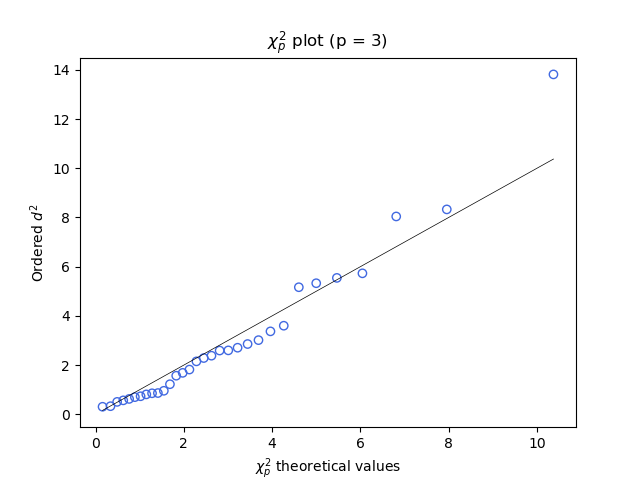
\includegraphics[scale=0.70]{./python/chapter-6/Exercise-6-17-d-chi2.png}
    \end{figure}

   \begin{center}
   \begin{tabular}{|l|l|}
        \hline
        \multicolumn{2}{|c|}{Mardia test} \\
        \hline
                & P-value \\
        \hline
        Skew     & 0.0    \\
        Kurtosis & 0.3604 \\
        \hline
   \end{tabular}
   \end{center}

   The $\chi^{2}$-plot shows some deviation from the line, which isn't promising.
    I also created code for the Mardia Multivariate normal test.
    The Mardia test is very significant for skewness and not significant for kurtosis.
    Since both tests are not significant, so we'd conclude that the data for the contrasts is not multivariate normal.
    
\end{enumerate}
